\documentclass[utf8, smaller, c]{beamer}

	\usepackage[mnf, foottitle]{citlab/beamerthemeCITlab}
	\usepackage{citlab/CITlab}
	\usepackage{citlab/CITlab_JM}
% 	\usepackage[utf8]{inputenc}
%   \usepackage[T1]{fontenc}
	\usepackage{lmodern}
	
	\usepackage{url}
	\usepackage{caption}
    \renewcommand{\figurename}{Abbildung}
    % \usepackage{hyperref}
    \usepackage{listings}
    \lstset{language=python, basicstyle=\footnotesize, tabsize=4, columns=fullflexible, xleftmargin=\parindent}
    \renewcommand{\tt}[1]{{\texttt{#1}}}
	
\begin{document}

	\author{M.Sc.~Johannes~Michael}
    \institute[Uni Rostock]{Universität Rostock}
	\date[22.~Oktober~2021]{Johannes Michael}
	\title{Mathematisches Praktikum}
	\subtitle{Grundlagen Python}

	\setbeamertemplate{footline}{\usebeamertemplate{firstFootline}}
	\frame{\maketitle}

	\setbeamertemplate{caption}{\insertcaption}
	\setbeamertemplate{footline}{\usebeamertemplate{allFootline}}

    \setbeamertemplate{section in toc}[ball unnumbered]
    \setbeamertemplate{subsection in toc}[square]
 	\frame{\tableofcontents}
 	
% Good resources:
% https://www.python-kurs.eu/python3_kurs.php
%
% http://www.coli.uni-saarland.de/courses/python1-10/folien/PythonI10-01.pdf
% http://www.coli.uni-saarland.de/courses/python1-10/folien/PythonI10-02.pdf
% . . .
% % http://www.coli.uni-saarland.de/courses/python1-10/folien/PythonI10-13.pdf

%%%%%%%%%%%%%%%%%%%%%%%%%%%%%%%%%%%%%%%%%%%%%%%%%%%%%%%%%%%%%%%%%%%%%%%%%%%%%%%%%%%%%%%%%
%%%%%%%%%%%%%%%%%%%%%%%%%%%%%%%%%%%%%%%%%%%%%%%%%%%%%%%%%%%%%%%%%%%%%%%%%%%%%%%%%%%%%%%%%
%%%%%%%%%%%%%%%%%%%%%%%%%%%%%%%%%%%%%%%%%%%%%%%%%%%%%%%%%%%%%%%%%%%%%%%%%%%%%%%%%%%%%%%%%
\section{Einführung}
\begin{frame}{Vorteile \& Besonderheiten}
	\begin{itemize}
		% notable features
		\item Open-source und plattformunabhängig
		\item Minimalistische Syntax
		\item Große Standardbibliothek
% 		\item Interaktiver Modus zum Testen kurzer Codeblöcke
% 		\item interpretierte Programmiersprache
		
		% programming-language features
		\item Unterstützt objektorientierte Programmierung
		\item Flexible Indizierung und Slicing bei Sequenzen
		\item Automatisches Speichermanagement
		\item $\cdots$
	\end{itemize}
\end{frame}

\begin{frame}{Interpreter \& Interaktive Shell}
	\begin{block}{Interpreter}
		Ein Interpreter (Softwaretechnik) ist ein Computerprogramm, das einen
		Programm-Quellcode im Gegensatz zu Assemblern oder Compilern nicht in eine auf dem
		System direkt ausführbare Datei übersetzt, sondern den Quellcode einliest,
		analysiert und ausführt.\footnote{\url{https://de.wikipedia.org/wiki/Interpreter}}
	\end{block}
	\vspace{-2mm}
	\begin{block}{Interaktive Shell}
		Die interaktive Shell steht zwischen dem Anwender und dem Betriebssystem bzw. dem
		zu interpretierenden Programm (z. B. Python). Eingaben werden dabei direkt von der
		Kommandozeile gelesen und unverzüglich ausgeführt. 
	\end{block}
\end{frame}

\begin{frame}[fragile]{Python--Skripte}
	\begin{itemize}
		\item Programme werden normalerweise nicht interaktiv eingetippt sondern in 
		Dateien/Skripten gespeichert.
		\item Skripte können mit beliebigem Texteditor bearbeitet werden\\$\longrightarrow$
		Empfehlung: PyCharm IDE
		\item Ausführen von Python Skripten:
		\begin{itemize}
			\item Direkt über IDE: \verb|Run...|
			\item Über Kommandozeile \verb|python script.py|
		\end{itemize}
%		\item Speichern der Ausgabe in externer Textdatei:
%		\begin{verbatim}
%		python skript.py > log_file.txt
%		\end{verbatim}
	\end{itemize}
	
\end{frame}

%%%%%%%%%%%%%%%%%%%%%%%%%%%%%%%%%%%%%%%%%%%%%%%%%%%%%%%%%%%%%%%%%%%%%%%%%%%%%%%%%%%%%%%%%
%%%%%%%%%%%%%%%%%%%%%%%%%%%%%%%%%%%%%%%%%%%%%%%%%%%%%%%%%%%%%%%%%%%%%%%%%%%%%%%%%%%%%%%%%
%%%%%%%%%%%%%%%%%%%%%%%%%%%%%%%%%%%%%%%%%%%%%%%%%%%%%%%%%%%%%%%%%%%%%%%%%%%%%%%%%%%%%%%%%
\section{Basisdatentypen \& Variablen}
\begin{frame}[fragile, allowframebreaks]{Basisdatentypen \& Variablen}
	\begin{block}{Datentyp}
		\begin{itemize}
			\item bezeichnet die Zusammenfassung konkreter Wertebereiche und die darauf definierten
			Operationen zu einer Einheit
			\item Basisdatentypen: Ganzzahlen (Integer), Fließkommazahlen (Float), Zeichenketten (Strings), Wahrheitswerte (Boolean)
		\end{itemize}
	\end{block}
	\vspace{2mm}
	\begin{itemize}
		\item in Programmiersprachen wie C/C++ oder Java muss der Datentyp explizit angegeben werden (Bindung an Datentyp)
		\begin{verbatim}
		int x = 50;         float y = 1.2;
		String s = "Test";  boolean b = true;
		\end{verbatim}
	\end{itemize}

	\pagebreak
	
	\vspace*{-2mm}
	\begin{itemize}
		\item Variablen halten keinen bestimmten Typ sondern referenzieren Objekte $\rightarrow$ keine Typdeklaration
		\begin{verbatim}
		x = 50               y = 1.2
		s = "Example Text"   b = True
		\end{verbatim}
		\item Zuweisung von Wert an Variable durch "="
		\begin{verbatim}		
		z = x + 10 
		\end{verbatim}
		\item Umwandlung von Datentypen (Casting): \\ \verb+x = 3.1 # Float+ \\ \verb+int(x)  # Integer, liefert 3+
	\end{itemize}
	
	\pagebreak	
	
	\vspace*{-2mm}
	\begin{itemize}
		\item Typ und Wert einer Variablen kann zur Laufzeit geändert werden (d.h. ein neues Objekt eines beliebigen Typs wird der Variablen zugewiesen)
		\item Variablen referenzieren Objekte und Objekte können einen beliebigen Datentyp haben $\rightarrow$ Variablen können nicht mit Datentypen "verknüpft" werden
		\item Typabfrage einer Variable:
		\begin{verbatim}
		x = 10
		print(type(x)) # <type 'int'>
		\end{verbatim}
	\end{itemize}
\end{frame}

%%%%%%%%%%%%%%%%%%%%%%%%%%%%%%%%%%%%%%%%%%%%%%%%%%%%%%%%%%%%%%%%%%%%%%%%%%%%%%%%%%%%%%%%%
%%%%%%%%%%%%%%%%%%%%%%%%%%%%%%%%%%%%%%%%%%%%%%%%%%%%%%%%%%%%%%%%%%%%%%%%%%%%%%%%%%%%%%%%%
%%%%%%%%%%%%%%%%%%%%%%%%%%%%%%%%%%%%%%%%%%%%%%%%%%%%%%%%%%%%%%%%%%%%%%%%%%%%%%%%%%%%%%%%%
\section{Operatoren}
\begin{frame}[fragile]{Operatoren}
	\begin{block}{Operatoren}
	\begin{itemize}
		\item \verb|+, -            :| Addition, Subtraktion
		\item \verb|*               :| Multiplikation
		\item \verb|/               :| Division (liefert \textit{float} Python3) 
		\item \verb|//              :| Ganzzahldivision (Ganzzahliger Anteil)
		\item \verb|**              :| Exponentiation
		\item \verb|%               :| Modulo (Rest)
		\item \verb|or, and, not    :| Boolsches \textit{Oder}, \textit{Und}, \textit{Nicht}
		\item \verb|is              :| Vergleichsoperator (Identität/Speicherort)
		\item \verb|<,<=,>,>=,!=,== :| (Standard-)Vergleichsoperatoren
		%\item \verb+|, \&, \^{}     :+ Bitweises textit{Oder}, \textit{Und}, \textit{XOR}
		%\item \verb|<<, >>          :| Shiftoperatoren ($x << y \Leftrightarrow x*2^y$, $x >> y \Leftrightarrow \frac{x}{2^y}$) 
	\end{itemize}
	\end{block}
\end{frame}

%%%%%%%%%%%%%%%%%%%%%%%%%%%%%%%%%%%%%%%%%%%%%%%%%%%%%%%%%%%%%%%%%%%%%%%%%%%%%%%%%%%%%%%%%
%%%%%%%%%%%%%%%%%%%%%%%%%%%%%%%%%%%%%%%%%%%%%%%%%%%%%%%%%%%%%%%%%%%%%%%%%%%%%%%%%%%%%%%%%
%%%%%%%%%%%%%%%%%%%%%%%%%%%%%%%%%%%%%%%%%%%%%%%%%%%%%%%%%%%%%%%%%%%%%%%%%%%%%%%%%%%%%%%%%
\section{Sequentielle Datentypen}
\begin{frame}[fragile, allowframebreaks]{Sequentielle Datentypen}
	\begin{itemize}
		\item Datentyp, der eine Folge von Elementen beinhaltet
		\item Elemente haben definierte Reihenfolge $\rightarrow$ Zugriff über Indizes möglich
		\item Python stellt \textit{Strings}, \textit{Listen} und \textit{Tupel} zur Verfügung
		\item Strings und Tupel sind nach Erzeugung \textit{unveränderlich} (immutable)
		\item Listen sind nach Erzeugung \textit{veränderlich} (mutable)
	\end{itemize}

	\pagebreak

	\begin{block}{Operationen auf Sequenzen}
	\begin{itemize}
		\item \verb+x in s   :+ prüft ob sich \tt{x} in \tt{s} befindet
		\item \verb|s + t    :| Verkettung von \tt{s} und \tt{t} als neue Sequenz
		\item \verb|s += t   :| hängt das Element \tt{t} an die Sequenz \tt{s} an
		\item \verb+s * n    :+ liefert \tt{n}--fache Kopie der Sequenz \tt{s}
		\item \verb+s[i]     :+ liefert das \tt{i}-te Element der Sequenz \tt{s}
		\item \verb+s[i:j]   :+ liefert Teilsequenz von Index \tt{i} bis Index \tt{j-1} von \tt{s}
		\item \verb+s[i:j:k] :+ wie \tt{s[i:j]}, nur jedes \tt{k}-te Element wird extrahiert
		\item \verb+len(s)   :+ liefert die Anzahl der Elemente in \tt{s}
		\item \verb+min(s)   :+ liefert das kleinste Element von \tt{s}
		\item \verb+max(s)   :+ liefert das größte Element von \tt{s}
	\end{itemize}
	\end{block}
\end{frame}

\begin{frame}[fragile, allowframebreaks]{Sequentielle Datentypen -- Strings}
	\begin{itemize}
		\item Sequenz von einzelnen Zeichen, die indiziert sind
		\item Indizierung beginnt bei 0 und ist von hinten möglich
			%\url{http://www.nltk.org/book_1ed/ch03.html}
			\center{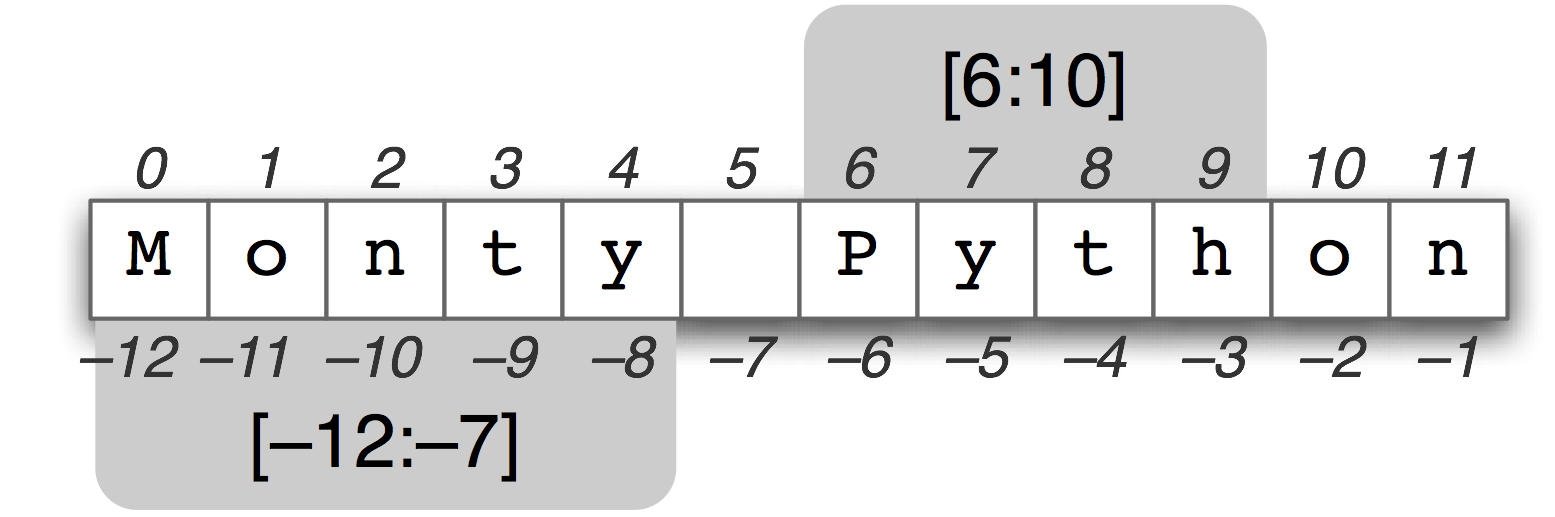
\includegraphics[scale=0.4]{pics/string-slicing.png}}
	\begin{verbatim}
	s = "Monty Python"
	print(s[0]) # Ausgabe: M
	\end{verbatim}
	\end{itemize}
	\begin{itemize}
		\item Strings sind unveränderlich: 
	\begin{verbatim}
	s[4] = "Y" # liefert Fehler
	\end{verbatim}
	\end{itemize}
	
	\pagebreak

	\begin{block}{String-Funktionen}
		\begin{itemize}
			\item Konkatenation:\newline
			\verb|"Monty" + " Python"| $\rightarrow$ \verb|"Monty Python"|
			\item Wiederholung:\newline
			\verb|"Python" * 3| $\rightarrow$ \verb|"PythonPythonPython"|
			\item Indexing:\newline
			\verb|"Monty Python"[-1]| $\rightarrow$ \verb|"n"|
			\item Slicing:\newline
			\verb|"Monty Python"[6:10]| $\rightarrow$ \verb|"Pyth"|
			\item Länge eines Strings:\newline
			\verb|len("Monty Python")| $\rightarrow$ \verb|12|
			\item Aufspalten von Strings:\newline
			\verb|"Monty Python".split()| $\rightarrow$ \verb|["Monty", "Python"]|
		\end{itemize}
	\end{block}
\end{frame}

%\begin{frame}[fragile]
%	\begin{itemize}
%		\item Escapezeichen sind Zeichenfolgen, die den Textfluss steuern:
%		\begin{itemize}
%			\item \textbackslash : Zeilenfortsetzung
%			\item \textbackslash n : Zeilenvorschub (Newline)
%			\item \textbackslash v : Vertikaler Tabulator
%			\item \textbackslash t : Horizontaler Tabulator
%			\item \textbackslash " : Doppeltes Anführungszeichen
%			\item \dots
%		\end{itemize}		 
% 	\end{itemize}
%\end{frame}

\begin{frame}[fragile, allowframebreaks]{Sequentielle Datentypen -- Listen}
	\begin{itemize}
		\item Eine Liste speichert eine Folge beliebiger Objekte
		\item Definiert über eckige Klammern und Elemente mit Kommas getrennt:
		\begin{verbatim}
		liste = ["Python", 4, 3.1]
		\end{verbatim}
		\item Listen sind veränderlich\newline
		\verb|liste[0] = 1| $\rightarrow$ \verb|[1, 4, 3.1]|
		\item \verb+liste[:]+ legt eine Kopie von \verb|liste| an
		\item \verb|[]| erzeugt leere Liste
		\item Liste von Listen ebenfalls möglich: \\ \verb|liste = [[1, 2, 3], [4, 5, 6]]|
	\end{itemize}

	\framebreak
	
	\vspace*{-2mm}
	\begin{itemize}
%	 	\item der "+=" Operator ist eine sehr gebräuchliche Methode zur Verkettung: \verb|s = s + t|
%	 	$\Longleftrightarrow$ \verb|s += t| 
%	 	\item += ist zeiteffizienter
		\item Operationen wie Konkatenation, Wiederholung, Indexing, Slicing, Länge $\dots$ übertragen sich analog
	 	\item Listeninhalt prüfen mittels \tt{in} und \tt{not in} Operatoren:
	 	\begin{verbatim}
	 	list = ["a", "b", "c", "d", "e"]
	 	"a" in list     # gibt Wert True zurück
	 	"d" not in list # gibt Wert False zurück
	 	s = "Python"
	 	"y" in s        # gibt Wert True zurück
	 	\end{verbatim}
	 	\vspace{-5mm}
	 	\item \textit{Tupel} entspricht unveränderlicher Liste (runde Klammern):
	 	\begin{verbatim}
	 	tuple = ("a", "b", "c", "d", "e")
		\end{verbatim}
	\end{itemize}

	\framebreak	
	
	\vspace*{-2mm}
	Eine Liste kann als ein Stapelspeicher (Stack) angesehen werden.
	\begin{block}{Operationen auf einem Stack}
		\begin{itemize}
			\item \verb+push+: legt neues Objekt auf den Stack \\
			$\rightarrow$ \verb+append+ als Äquivalent für Listen
			\item \verb+pop+: gibt oberstes Objekt des Stacks zurück und entfernt es \\
			$\rightarrow$ \verb+liste.pop(i)+ wendet \verb+pop+ auf das i-te Element an
			\item \verb+peek+: gibt oberstes Objekt des Stacks zurück ohne es zu entfernen $\rightarrow$
			\verb+liste[-1]+ als Äquivalent für Listen
		\end{itemize}
	\end{block}

	\framebreak

	\begin{block}{\tt{append} vs \tt{extend}}
		\begin{itemize}
			\item Hinzufügen von mehr als einem Element:
			\begin{verbatim}
				l = [1, 2, 3]
				l.append([4, 5])	# ergibt [1, 2, 3, [4, 5]]
			\end{verbatim}
			\item verwende stattdessen \tt{extend}:
			\begin{verbatim}
				l.extend([4, 5])	# ergibt [1, 2, 3, 4, 5]
			\end{verbatim}				 
			\item das Argument von \tt{extend} muss ein iterierbares Objekt sein:
			\begin{verbatim}
				l.extend("Hello")	
				# ergibt [1, 2, 3, 'H', 'e', 'l', 'l', 'o']
			\end{verbatim}
		\end{itemize}
	\end{block}

	\framebreak

	\begin{block}{remove}
		\begin{itemize}
			\item Entfernen eines Wertes ohne Kenntnis des Indexes:
			\begin{verbatim}
				abc = ["a", "b", "c", "d", "e"]
				abc.remove("b")		# abc = ["a", "c", "d", "e"]
			\end{verbatim}
			\item Fehler falls das Element nicht in der Liste vorkommt:
			\begin{verbatim}
				abc.remove("f")
				ValueError: list.remove(x): x not in list
			\end{verbatim}
		\end{itemize}
	\end{block}
	\vspace{-2mm}
	\begin{block}{index}
		\begin{itemize}
			\item Finden der Position eines Elementes:
			\begin{verbatim}
				abc = ["a", "b", "c", "a", "e"]
				abc.index("a")        # gibt 0 zurück
				abc.index("a", 1)     # gibt 3 zurück
				abc.index("a", 1, 2)  # ValueError
			\end{verbatim}
		\end{itemize}
	\end{block}

	\framebreak

	\begin{block}{insert}
		\begin{itemize}
			\item Es ist nicht möglich mittels \verb+append+ ein Element an beliebiger Stelle einzufügen $\rightarrow$ 
			\verb+insert+:
			\begin{verbatim}
				abc = ["a", "b", "c", "e"]
				abc.insert(3, "d")
				# abc = ["a", "b", "c", "d", "e"]
			\end{verbatim}
		\end{itemize}
	\end{block}
\end{frame}

%%%%%%%%%%%%%%%%%%%%%%%%%%%%%%%%%%%%%%%%%%%%%%%%%%%%%%%%%%%%%%%%%%%%%%%%%%%%%%%%%%%%%%%%%
%%%%%%%%%%%%%%%%%%%%%%%%%%%%%%%%%%%%%%%%%%%%%%%%%%%%%%%%%%%%%%%%%%%%%%%%%%%%%%%%%%%%%%%%%
%%%%%%%%%%%%%%%%%%%%%%%%%%%%%%%%%%%%%%%%%%%%%%%%%%%%%%%%%%%%%%%%%%%%%%%%%%%%%%%%%%%%%%%%%
\section{Dictionaries}
\begin{frame}[fragile, allowframebreaks]{Dictionaries}
	\vspace*{-2mm}
	\begin{block}{Assoziatives Datenfeld}
		Das assoziative Datenfeld (englisch map, dictionary) ist eine Datenstruktur, die --
		anders als ein gewöhnliches Feld (engl. array) – nichtnumerische (oder nicht fortlaufende) Schlüssel (zumeist
		Zeichenketten) verwendet, um enthaltene Elemente zu adressieren.
		\footnote{\url{https://de.wikipedia.org/wiki/Assoziatives_Datenfeld}}
	\end{block}
	\begin{itemize}
		\item besteht aus Schlüssel-Objekt-Paaren (key-value pairs)
		\item zu einem Schlüssel gehört immer ein Objekt (Mapping)
		\item Nicht sequentiell $\rightarrow$ keine Anordnung, keine Indizierung
		\item Zugriff über Schlüssel
	\end{itemize}

	\pagebreak

	\begin{block}{Beispiele}
		\begin{itemize}
			\item Leeres Dictionary: \verb+d = {}+
			\item Englisch-Deutsch Wörterbuch:
			\begin{verbatim}
			ed = {"red":"rot", "green":"grün"}	
			\end{verbatim}	
			\item Deutsch-Französisch Wörterbuch:
			\begin{verbatim}
			df = {"rot":"rouge", "grün":"vert"}
			\end{verbatim}
			\item Englisch-Französisch Wörterbuch über Transitiviät:
			\begin{verbatim}
			df[ed["red"]]   # gibt "rouge" zurück
			\end{verbatim}											
		\end{itemize}
	\end{block}
	\begin{itemize}
		\item als Werte können beliebige Typen verwendet werden
		\item bei Schlüsseln können nur Instanzen \textbf{unveränderlicher} Datentypen verwendet werden (z. B. Strings)
	\end{itemize}

	\pagebreak
	
	\begin{block}{Operatoren auf Dictionaries}
		\begin{itemize}
			\item \verb+len(d)       :+ liefert die Anzahl der Schlüssel-Werte-Paare
			\item \verb+del d[k]     :+ löscht Eintrag zum Schlüssel \tt{k}
			\item \verb+k (not) in d :+ True, wenn es in \tt{d} (k)einen Schlüssel \tt{k} gibt
		\end{itemize}
	\end{block}
	\vspace{-2mm}
	\begin{block}{\tt{pop}}
		\verb+pop+ existiert in abgewandelter Form auch für Dictionaries:
		\begin{verbatim}
		d = {"a":1, "b":2, "c":3}
		d.pop("a")    # gibt Wert 1 zurück
		              # d = {"b":2, "c":3}
		d.pop("d")    # KeyError: 'd'
		d.pop("d", 4) # gibt Default-Wert 4 zurück
		d.pop("b", 4) # gibt Wert 2 zurück
		\end{verbatim}
	\end{block}

	\pagebreak
	
	\begin{block}{\tt{popitem}}
		\verb+popitem+ benötigt keine Parameter und liefert beliebiges Schlüssel-Wert-Paar als Tupel zurück:
		\begin{verbatim}
		d = {"a":1, "b":2, "c":3}
		d.popitem()  # gibt z. B. ("a", 1) zurück
		             # d = {"b":2, "c":3}
		\end{verbatim}
	\end{block}
	\vspace{-2mm}
	\begin{block}{\tt{get}}
	\verb+get+ als weitere Methode um auf die Werte über die Schlüssel zuzugreifen:
		\begin{verbatim}
		d = {"a":1, "b":2, "c":3}
		d.get("c")  # gibt Wert 3 zurück
		d["c"]      # äquivalent
		\end{verbatim}
	\end{block}

	\pagebreak

	\begin{block}{\tt{copy}}
		\begin{itemize}
			\item \verb+copy+ ermöglicht das Kopieren von Dictionaries:
			\begin{verbatim}
			d1 = {"a":1, "b":2, "c":3}
			d2 = d1.copy()   # d2 = {"a":1, "b":2, "c":3}
			d1["a"] = 4      # d1 = {"a":4, "b":2, "c":3}
			                 # d2 = {"a":1, "b":2, "c":3}
			\end{verbatim}
			\item falls es sich bei dem Wert um einen komplexen Datentyp handelt, wirken sich Änderungen innerhalb
			eines solchen Wertes auf Original und Kopie aus:
			\begin{verbatim}
			d1 = {"a":[1,2], "b":[3,4]}
			d2 = d1.copy() # d2 = {"a":[1,2], "b":[3,4]}
			d1["a"][0] = 5 # d1=d2 = {"a":[5,2], "b":[3,4]}  
			\end{verbatim}
		\end{itemize}
	\end{block}

	\pagebreak

	\begin{block}{\tt{clear}}
		\verb+clear+ leert den Inhalt eines Dictionaries (das Dictionary wird dabei nicht gelöscht):
		\begin{verbatim}
		d = {"a":1, "b":2, "c":3}
		d.clear  # d = {}
		\end{verbatim}
	\end{block}
	\begin{block}{\tt{update}}
		\verb+update+ ermöglicht das Updaten über weitere Dictionaries:
		\begin{verbatim}
		d1 = {"a":1, "b":2}
		d2 = {"b":3, "c":4}
		d1.update(d2)  # d1 = {"a":1, "b":3, "c":4}
		\end{verbatim}
	\end{block}

	\pagebreak

	\begin{block}{Iteration über Dictionaries}
		\begin{itemize}
			\item Iteration über die Schlüssel: 
			\begin{verbatim}
			d = {"a":1, "b":2}
			for key in d:  # liefert nacheinander 'a' und 'b'
			  print(key)
			\end{verbatim}
			\vspace*{2mm}
			oder
			\vspace*{2mm}
			\begin{verbatim}
			for key in d.keys():
			  print(key)
			\end{verbatim}
			\item Iteration über die Werte:
			\begin{verbatim}
			d = {"a":1, "b":2}
			for val in d.values():  # liefert nacheinander
			  print(val)            # 1 und 2
			\end{verbatim}
		\end{itemize}
	\end{block}

	\pagebreak

	\begin{block}{Casting zwischen Listen und Dictionaries}
		\begin{itemize}
			\item Dictionary $\rightarrow$ Liste:
			\begin{verbatim}
			d = {"a":1, "b":2, "c":3}
			l_keys = list(d) # oder l_keys = d.keys()
			l_values = d.values()
			\end{verbatim}
			\item Liste $\rightarrow$ Dictionary:
			\begin{verbatim}
			l1 = ["a", "b", "c"]
			l2 = [1, 2, 3]
			d = dict(zip(l1,l2))
			# zip fasst die Komponenten zu Tupeln zusammen
			# d = {"a":1, "b":2, "c":3}
			\end{verbatim}
		\end{itemize}
	\end{block}
\end{frame}

%%%%%%%%%%%%%%%%%%%%%%%%%%%%%%%%%%%%%%%%%%%%%%%%%%%%%%%%%%%%%%%%%%%%%%%%%%%%%%%%%%%%%%%%%
%%%%%%%%%%%%%%%%%%%%%%%%%%%%%%%%%%%%%%%%%%%%%%%%%%%%%%%%%%%%%%%%%%%%%%%%%%%%%%%%%%%%%%%%%
%%%%%%%%%%%%%%%%%%%%%%%%%%%%%%%%%%%%%%%%%%%%%%%%%%%%%%%%%%%%%%%%%%%%%%%%%%%%%%%%%%%%%%%%%
\section{Formatierte Ausgaben}
\begin{frame}[fragile, allowframebreaks]{Formatierte Ausgaben}
	\begin{itemize}
		\item Einfachste Ausgabe: Kommaseparierte Liste von Werten.
	\end{itemize}
	\begin{lstlisting}
		a, b, c = 1, 2.2, "test"
		print(a, a+b, c)
	\end{lstlisting}
	\begin{itemize}
		\item Ausgabeseparator und Endzeichen kann explizit gesetzt werden.
	\end{itemize}
	\begin{lstlisting}
		print(a, a+b, c, sep=",", end="|")
	\end{lstlisting}
	\begin{itemize}
		\item Alternativ: Neuen String mittels String-Konkatenation ausgeben (beachte dass Variablen in Strings umgewandelt werden müssen).
	\end{itemize}
	\begin{lstlisting}
		print(str(a) + "," + str(a+b) + "," + c)
	\end{lstlisting}
	
	\pagebreak
	
	\vspace*{-2mm}
	\begin{itemize}
		\item "Veraltet": \textbf{String-Modulo-Operator}.
		\item Syntax: "Format-String mit Platzhaltern" \% (Füllwerte)
		\item Platzhalter: \%[flags][width][.precision]type
	\end{itemize}
	\begin{figure}[hb]
		\centering
		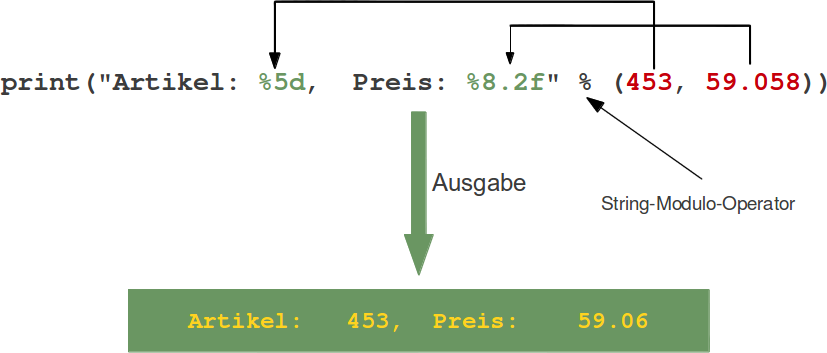
\includegraphics[width=0.7\textwidth]{pics/formatierte_ausgabe1.png}
		{\tiny\url{https://www.python-kurs.eu/python3_formatierte_ausgabe.php}}
	\end{figure}
	
	
	\pagebreak
	
	\vspace*{-2mm}
	\begin{itemize}
		\item "Klassisch": String-Methode \textbf{format}
		\item Syntax: "Format-String mit Format-Codes".format(Füllwerte)
		\item Format-Codes: \{[index]:[[fill]align][flag][width][.precision][type]\}
	\end{itemize}
	\begin{figure}[hb]
		\centering
		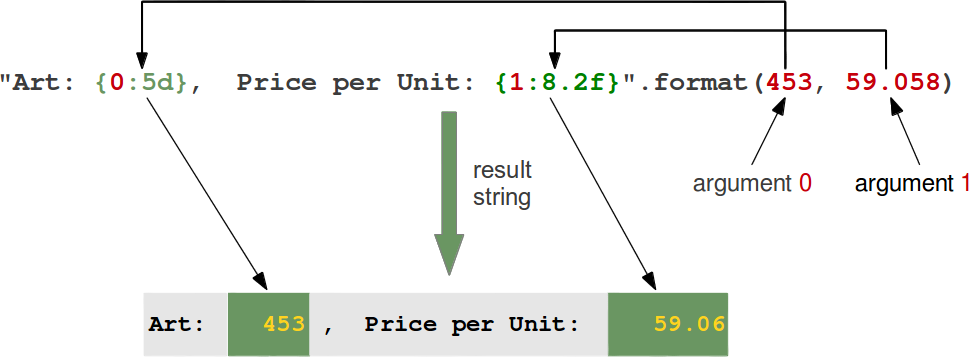
\includegraphics[width=0.8\textwidth]{pics/formatierte_ausgabe2.png}
		{\tiny\url{https://www.python-kurs.eu/python3_formatierte_ausgabe.php}}
	\end{figure}
	
	\pagebreak
	
	\vspace*{-2mm}
	\begin{itemize}
		\item "Neu": \textbf{f-Strings}
		\item Analog zu format-Strings, wobei Variablen in Format-Codes integriert werden und String mit einem 'f' deklariert wird
	\end{itemize}
	\begin{lstlisting}
		x = 30.8
		p = 3.141592
		print("First value = {:.2f}, Second value = {:.4f}".format(x, p))
		print(f"First value = {x:.2f}, Second value = {p:.4f}")
	\end{lstlisting}
	
	\pagebreak
	
	\vspace*{-2mm}
	\begin{tabular}{|p{1.2cm}|p{8.5cm}|} \hline
		\textbf{type} & \textbf{Bedeutung} \\ \hline
		'b' & Integer, binär. \\ \hline
		'd' & Integer, dezimal. \\ \hline
		'o' & Integer, oktal. \\ \hline
		'x', 'X' & Integer, hexadezimal (Klein- bzw. Großbuchstaben). \\ \hline
		'c' & Zum Integer gehörendes Unicode-Zeichen. \\ \hline
		'f' & Float. \\ \hline
		'e', 'E' & Float, Exponentialformat (Klein- bzw. Großbuchstaben). \\ \hline
		'g', 'G' & adaptiv 'f' oder 'e' bzw. 'E'. \\ \hline
		's' & Umwandlung in einen String mittels str()-Methode. \\ \hline
		'\%' & Umwandlung in Prozent und zusätzliches \%-Zeichen. \\ \hline
	\end{tabular}
	
	\pagebreak
	
	\vspace*{-2mm}
	\begin{itemize}
		\item index: Positions- oder Schlüsselwortparameter
		\item fill: beliebiges Füllzeichen
	\end{itemize}
	\begin{tabular}{|p{0.9cm}|p{8.5cm}|} \hline
		\textbf{align} & \textbf{Bedeutung} \\ \hline
		'<' & Feld wird linksbündig ausgegeben (Standard für Strings). \\ \hline
		'>' & Feld wird rechtsbündig ausgegeben (Standard für numerische Werte). \\ \hline
		'\^{}' & Feld wird zentriert ausgegeben. \\ \hline
		'=' & Füllzeichen werden zwischen dem Vorzeichen (falls existent) und der Zahl ausgegeben. Kann nur auf numerische Werte angewendet werden. \\ \hline
	\end{tabular}
	
	\pagebreak
	
	\vspace*{-2mm}
	\begin{itemize}
		\item width: totale Anzahl an auszugebenden Zeichen
		\item precision: Präzision des Dezimalanteils
	\end{itemize}
	\begin{tabular}{|p{0.9cm}|p{8.5cm}|} \hline
		\textbf{flag} & \textbf{Bedeutung} \\ \hline
		'+' & Ausgabe von positiven und negativen Vorzeichen. \\ \hline
		'-' & Ausgabe von negativen Vorzeichen (Standard). \\ \hline
		' ' & Bei keinem Vorzeichen wird ein Leerzeichen vorangestellt. \\ \hline
		'0' & Auffüllen mit Nullen unter Beachtung eines möglichen Vorzeichens (entspricht align '=' und fill '0'). \\ \hline
		',' & Tausender Gruppierungen durch Komma getrennt. \\ \hline
		'\#' & Binär-, Oktal- und Hexadezimalsystem werden mit einem Präfix versehen. \\ \hline
	\end{tabular}
\end{frame}

%%%%%%%%%%%%%%%%%%%%%%%%%%%%%%%%%%%%%%%%%%%%%%%%%%%%%%%%%%%%%%%%%%%%%%%%%%%%%%%%%%%%%%%%%
%%%%%%%%%%%%%%%%%%%%%%%%%%%%%%%%%%%%%%%%%%%%%%%%%%%%%%%%%%%%%%%%%%%%%%%%%%%%%%%%%%%%%%%%%
%%%%%%%%%%%%%%%%%%%%%%%%%%%%%%%%%%%%%%%%%%%%%%%%%%%%%%%%%%%%%%%%%%%%%%%%%%%%%%%%%%%%%%%%%
\section{Code--Strukturierung}
\begin{frame}[fragile]{Code-Strukturierung}
	\begin{itemize}
		\item Anstelle von Schlüsselwörtern oder speziellen Klammern, dient die \textbf{Einrückung von Zeilen} als Strukturierungselement
		\item Codeblöcke setzen sich häufig aus einem Anweisungskopf und einem Anweisungskörper zusammen
	\end{itemize}
	\begin{lstlisting}
		Anweisungskopf:
			Anweisung
				...
			Anweisung
	\end{lstlisting}
	\begin{itemize}
		\item Wesentlich ist der Doppelpunkt am Ende des Kopfes und die gleichmäßige Einrückung des Anweisungskörpers
		\item Codeblöcke können geschachtelt werden
	\end{itemize}
\end{frame}

%%%%%%%%%%%%%%%%%%%%%%%%%%%%%%%%%%%%%%%%%%%%%%%%%%%%%%%%%%%%%%%%%%%%%%%%%%%%%%%%%%%%%%%%%
%%%%%%%%%%%%%%%%%%%%%%%%%%%%%%%%%%%%%%%%%%%%%%%%%%%%%%%%%%%%%%%%%%%%%%%%%%%%%%%%%%%%%%%%%
%%%%%%%%%%%%%%%%%%%%%%%%%%%%%%%%%%%%%%%%%%%%%%%%%%%%%%%%%%%%%%%%%%%%%%%%%%%%%%%%%%%%%%%%%
\section{Bedingte Anweisungen}
\begin{frame}[fragile, allowframebreaks]{Bedingte Anweisungen}
	\begin{itemize}
		\item	Eine \textbf{bedingte Anweisung} oder \textbf{Verzweigung} ist ein Codeteil, der nur unter bestimmten Bedingungen ausgeführt wird.
		\item Bedingte Anweisungen können geschachtelt werden.
	\end{itemize}
	\begin{block}{\tt{if}-Anweisung}
		\begin{lstlisting}
		if bedingung:
			anweisung_1
			anweisung_2
				...
		\end{lstlisting}
		\begin{itemize}
			\item Der eingerückte Block wird nur dann ausgeführt wenn die Bedingung \textit{bedingung} zutrifft, also logisch \textit{true} liefert.
		\end{itemize}
	\end{block}
	\pagebreak
	\begin{block}{\tt{elif}- und \tt{else}-Anweisung}
		\begin{itemize}
			\item Optionale Erweiterungen der \tt{if}-Anweisung.
		\end{itemize}
		\begin{lstlisting}
		if bedingung_1:
			anweisung_1
		elif bedingung_2:
			anweisung_2
		# weitere elif-Anweisungen
		else:
			anweisung_n
		\end{lstlisting}
		\begin{itemize}
			\item Die \tt{elif}-Anweisung hat die gleiche Funktionalität wie die \tt{if}-Anweisung, wird aber nur geprüft wenn die Bedingung des vorherigen \tt{elif} oder \tt{if} \textit{false} war.
			\item Die \tt{else}-Anweisung wird am Ende ausgeführt wenn keine vorherige Bedingung eingetroffen ist.
		\end{itemize}
	\end{block}
\end{frame}

%%%%%%%%%%%%%%%%%%%%%%%%%%%%%%%%%%%%%%%%%%%%%%%%%%%%%%%%%%%%%%%%%%%%%%%%%%%%%%%%%%%%%%%%%
%%%%%%%%%%%%%%%%%%%%%%%%%%%%%%%%%%%%%%%%%%%%%%%%%%%%%%%%%%%%%%%%%%%%%%%%%%%%%%%%%%%%%%%%%
%%%%%%%%%%%%%%%%%%%%%%%%%%%%%%%%%%%%%%%%%%%%%%%%%%%%%%%%%%%%%%%%%%%%%%%%%%%%%%%%%%%%%%%%%
\section{Schleifen}
\begin{frame}[fragile, allowframebreaks]{Schleifen}
	\begin{itemize}
		\item \textbf{Schleifen} ermöglichen es einen Codeblock wiederholt auszuführen, solange das \textit{Schleifenkriterium} erfüllt ist.
	\end{itemize}
	\begin{minipage}[h]{0.4\textwidth}
		\begin{itemize}
			\item das Schleifenkriterium kann bspw. durch einen Zähler, eine explizite Bedingung oder durch das Durchlaufen einer Sammlung definiert sein.
		\end{itemize}
	\end{minipage}
	\hfill
	\begin{minipage}[h]{0.58\textwidth}
		\begin{figure}[hb]
		    \centering
			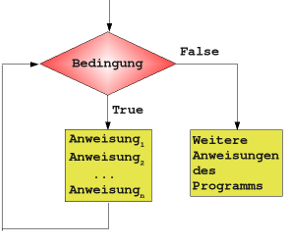
\includegraphics[scale=0.6]{pics/schleife1.png}
			{\tiny\url{https://www.python-kurs.eu/python3_schleifen.php}}
		\end{figure}
	\end{minipage}
	\begin{itemize}
		\item Schleifen können geschachtelt werden.
	\end{itemize}
	\pagebreak
	\begin{block}{\tt{while}-Schleife}
		\begin{itemize}
			\item Die \tt{while}-Schleife wiederholt den eingerückten Codeblock solange die Bedingung \textit{true} liefert.
			\item Sobald die Bedingung \textit{false} liefert wird die Schleife verlassen bzw. der optionale \tt{else}-Zweig aufgerufen
		\end{itemize}
		\begin{minipage}[h]{0.4\textwidth}
			\begin{lstlisting}
			while bedingung:
				anweisung_1
					...
				anweisung_n
			else:
				anweisung_else
			\end{lstlisting}
		\end{minipage}
		\hfill
		\begin{minipage}[h]{0.58\textwidth}
		\begin{figure}[hb]
		    \centering
			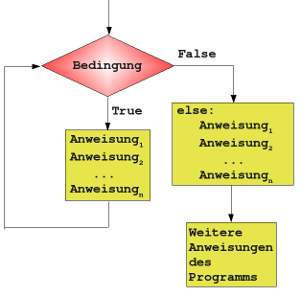
\includegraphics[scale=0.45]{pics/schleife2.png}
			{\tiny\url{https://www.python-kurs.eu/python3_schleifen.php}}
		\end{figure}
	\end{minipage}
	\end{block}
	\pagebreak
	\begin{block}{\tt{break}- und \tt{continue}-Anweisung}
		\begin{itemize}
			\item Die \tt{break}-Anweisung terminiert sofort die Schleife in der sie enthalten ist (bei geschachtelten Schleifen nur die innerste).
			\item Die \tt{continue}-Anweisung beendet lediglich den aktuellen Durchlauf und kehrt zum Schleifenkopf zurück.
		\end{itemize}
		\begin{minipage}[h]{0.4\textwidth}
			\begin{lstlisting}[basicstyle=\footnotesize]
			while bedingung_1:
				anweisung_1
				if bedingung_2:
					break
				elif bedingung_3:
					continue
				else:
				anweisung_2
			else:
				anweisung_3
			\end{lstlisting}
		\end{minipage}
		\hfill
		\begin{minipage}[h]{0.58\textwidth}
			\begin{figure}[hb]
			    \centering
				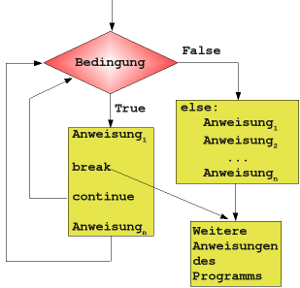
\includegraphics[scale=0.4]{pics/schleife3.png}
				{\tiny\url{https://www.python-kurs.eu/python3_schleifen.php}}
			\end{figure}
		\end{minipage}
	\end{block}
	\pagebreak
	\begin{block}{\tt{for}-Schleife}
		\begin{itemize}
			\item Pythons Art von \tt{for}-Schleife entspricht einer \textbf{for-each}-Schleife: Iteration über eine Sequenz von Objekten.
		\end{itemize}
		\begin{lstlisting}[basicstyle=\footnotesize]
		for var in sequenz:
		    anweisung_1
		        ...
		    anweisung_n
		else:
			anweisung_else
		\end{lstlisting}
		\begin{itemize}
			\item Bei jedem Schleifendurchlauf wird das nächste Element der Sequenz der Variablen \textit{var} zugewiesen.
			\item Die Schleife terminiert, sobald das letzte Element der Sequenz durchlaufen wurde.
		\end{itemize}
	\end{block}
	\pagebreak
	\begin{block}{\tt{range}-Funktion}
		\begin{itemize}
			\item Simulation von Zählschleifen mittels der \tt{range}-Funktion.
			\item \tt{range([begin,]end[,step])}\\ liefert einen Iterator über Zahlen im Bereich von 0 bzw. \textit{begin} (inklusive) bis \textit{end} (exklusive) mit Schrittweite 1 bzw. \textit{step}.
			\item Zählschleife von 1 bis 100:
		\end{itemize}
		\begin{lstlisting}
		for counter in range(1, 101):
			anweisung_1
				...
			anweisung_n
		\end{lstlisting}
	\end{block}
\end{frame}

%%%%%%%%%%%%%%%%%%%%%%%%%%%%%%%%%%%%%%%%%%%%%%%%%%%%%%%%%%%%%%%%%%%%%%%%%%%%%%%%%%%%%%%%%
%%%%%%%%%%%%%%%%%%%%%%%%%%%%%%%%%%%%%%%%%%%%%%%%%%%%%%%%%%%%%%%%%%%%%%%%%%%%%%%%%%%%%%%%%
%%%%%%%%%%%%%%%%%%%%%%%%%%%%%%%%%%%%%%%%%%%%%%%%%%%%%%%%%%%%%%%%%%%%%%%%%%%%%%%%%%%%%%%%%
\section{Funktionen}
\begin{frame}[fragile, allowframebreaks]{Funktionen}
	\begin{itemize}
		\item Strukturelement zur Gruppierung von Anweisungen $\rightarrow$ Codewiederverwendung und verbesserte Verständlichkeit
	\end{itemize}
	\begin{lstlisting}
	def funktionsname(parameterliste):
		"""docstring"""
		anweisung(en)
		[return objekt(e)]
	\end{lstlisting}
	\begin{itemize}
		\item Parameterliste kann beliebig viele Argumente enthalten.
		\item Parameter können obligatorisch und optional sein (letztere werden bei fehlender Übergabe durch Default-Werte ersetzt).
		\item (optionale) \textbf{return}-Anweisung beendet Funktionsaufruf und liefert das(die) zugehörige(n) Objekt(e) bzw. \textit{None} zurück.
	\end{itemize}
	
	\pagebreak
	
	\begin{block}{Parameter}
		\begin{itemize}
			\item Obligatorische Parameter:
		\end{itemize}
		\begin{lstlisting}
	def greet(name):
		print(f"Hello {name}!")
		\end{lstlisting}
		\begin{itemize}
			\item Optionale Parameter mit Default-Werten:
		\end{itemize}
		\begin{lstlisting}
	def greet(name="everybody"):
		print(f"Hello {name}!")
		\end{lstlisting}
		\begin{itemize}
			\item Funktionenaufruf mittels Schlüsselwortparameter:
		\end{itemize}
		\begin{lstlisting}
	def my_function(a, b, c=0, d=0):
		return a + b - c - d
	print(my_function(5, 10, d=2))
		\end{lstlisting}
	\end{block}
	
    \pagebreak
    
    \begin{itemize}
        \item Funktionen können mit globalen und lokalen Objekten arbeiten
        \item[$\rightarrow$] Lokal definierte Objekte sind für den globalen Kontext nicht sichtbar
        \item[$\rightarrow$] Zum Ändern globaler Objekte (anstatt nur zu referenzieren), müssen diese mit \tt{global} gekennzeichnet werden
    \end{itemize}
    \begin{lstlisting}
        global_var = 0
        def func(integer):
            global global_var
            local_var = integer ** 2
            print(global_var)
            global_var += local_var  # needs 'global' keyword
        func(10)
        print(global_var)
        # print(local_var)  # Error
    \end{lstlisting}
	
	\pagebreak
	
	\begin{block}{Variable Parameteranzahl}
	\begin{itemize}
		\item Tupel-Referenz "*" fasst Parameter zu einem Tupel zusammen:
	\end{itemize}
	\begin{lstlisting}
	def func(*params):
		print(params)
	func("My", "answer", "is", 42)
	\end{lstlisting}
	\begin{itemize}
		\item Beliebige Schlüsselwortparameter mittels "**":
	\end{itemize}
	\begin{lstlisting}
	def func(**key_vals):
		print(key_vals)
	func(de="German", en="English", fr="French")
	\end{lstlisting}
	\begin{itemize}
		\item Beachte Semantik von "*" und "**" in Funktionsdefinitionen bzw. -aufrufen: Dienen dem Packen bei Funktionsdefinitionen und Entpacken bei Funktionsaufrufen.
	\end{itemize}
	\end{block}
	
% 	\pagebreak
	
% 	\begin{block}{Funktionen in Funktionen}
% 		\begin{itemize}
% 			\item Verschachtelte Funktionen (lokale Funktionsdefinitionen innerhalb einer Funktion):
% 		\end{itemize}
% 		\begin{lstlisting}
% 	def f():
% 		def g():
% 			print("Hello, it's 'g'.")
% 			print("Thanks for calling me.")
% 		print("This is 'f'.")
% 		print("We'll call 'g' now.")
% 		g()
% 	f()
% 		\end{lstlisting}
% 	\end{block}
	
% 	\pagebreak
	
% 	\begin{block}{Funktionen als Parameter}
% 		\begin{itemize}
% 			\item Funktionen sind Objekte und können somit referenziert werden.
% 		\end{itemize}
% 		\begin{lstlisting}
% 	def g():
% 		print("Hello, it's 'g'.")
% 		print("Thanks for calling me.")
		
% 	def f(func):
% 		print("This is 'f'.")
% 		print(f"We'll call {func.__name__} now.")
% 		func()
		
% 	f(g)
% 		\end{lstlisting}
% 	\end{block}
	
% 	\pagebreak
	
% 	\begin{block}{Funktionen als Rückgabe}
% 		\begin{itemize}
% 			\item Rückgaben einer Funktion referenzieren Objekte $\rightarrow$ Referenzen auf Funktionen können zurückgegeben werden.
% 		\end{itemize}
% 		\begin{lstlisting}
% 	def f(x):
% 		def g(y):
% 			return y+x
% 		return g
		
% 	f1 = f(1)
% 	f5 = f(5)
% 	print(f1(10))
% 	print(f5(10))
% 		\end{lstlisting}	
% 	\end{block}
\end{frame}

%%%%%%%%%%%%%%%%%%%%%%%%%%%%%%%%%%%%%%%%%%%%%%%%%%%%%%%%%%%%%%%%%%%%%%%%%%%%%%%%%%%%%%%%%
%%%%%%%%%%%%%%%%%%%%%%%%%%%%%%%%%%%%%%%%%%%%%%%%%%%%%%%%%%%%%%%%%%%%%%%%%%%%%%%%%%%%%%%%%
%%%%%%%%%%%%%%%%%%%%%%%%%%%%%%%%%%%%%%%%%%%%%%%%%%%%%%%%%%%%%%%%%%%%%%%%%%%%%%%%%%%%%%%%%
\section{Dateien}
\begin{frame}[fragile, allowframebreaks]{Dateien}
	\begin{block}{Text aus Datei lesen}
		\begin{itemize}
			\item \tt{open}-Funktion erzeugt Dateiobjekt und liefert Referenz auf dieses Objekt.
		\end{itemize}
		\begin{lstlisting}
	open(filename[, mode][, encoding])
		\end{lstlisting}
		\begin{itemize}
			\item Datei zum Lesen öffnen: \textit{mode} = "r" (read, default)
		\end{itemize}
		\begin{lstlisting}
	txtfile = open("input.txt", "r")
		\end{lstlisting}
		\begin{itemize}
			\item Zeilenweises Einlesen mittels \tt{for}-Schleife:
		\end{itemize}
		\begin{lstlisting}
	for line in txtfile:
		print(line.rstrip())
		\end{lstlisting}
		\begin{itemize}
		    \item Kodierung beachten (z.B. für Umlaute)!
		\end{itemize}
	\end{block}
	
	\pagebreak
	
	\begin{block}{Datei schließen}
		\begin{itemize}
			\item \tt{close}-Funktion schließt Datei nach ihrer Bearbeitung:
		\end{itemize}
		\begin{lstlisting}
	txtfile.close()
		\end{lstlisting}
		\begin{itemize}
			\item Alternativ benutzt man die Datei innerhalb eines \tt{with}-Blocks:
		\end{itemize}			
		\begin{lstlisting}
	with open("input.txt", "r") as txtfile:
		for line in txtfile:
			print(line.rstrip())
		\end{lstlisting}
		\begin{itemize}
			\item Nach Verlassen des \tt{with}-Blocks wird die Datei automatisch geschlossen.
		\end{itemize}
	\end{block}
	
	\begin{block}{Schreiben in Datei}
		\begin{itemize}
			\item Datei zum Schreiben öffnen: \textit{mode} = "w" (write).
			\item \tt{write}-Funktion schreibt Daten in Datei.
		\end{itemize}
		\begin{lstlisting}
	in_file = open("input.txt", "r")
	out_file = open("output.txt", "w")
	i = 1
	for line in in_file:
		out_file.write(str(i) + ": " + line)
		i += 1
	in_file.close()
	out_file.close()
		\end{lstlisting}
		\begin{itemize}
			\item Achtung: \textit{mode} = "w" löscht die Datei beim Öffnen! Nutze \textit{mode} = "a" zum Anhängen von Daten.
		\end{itemize}
	\end{block}
	
	\pagebreak
	
	\begin{block}{Komplettes Einlesen}
		\begin{itemize}
			\item Datei in eine komplette Datenstruktur einlesen.
			\begin{itemize}
				\item \tt{readlines}-Funktion liefert eine Liste zurück.
				\item \tt{read}-Funktion liefert einen String zurück.
			\end{itemize}
		\end{itemize}
		\begin{lstlisting}
	text_list = open("input.txt").readlines()
	text_string = open("input.txt").read()
	
	print(text_list)
	print(text_string)
		\end{lstlisting}
	\end{block}
\end{frame}

%%%%%%%%%%%%%%%%%%%%%%%%%%%%%%%%%%%%%%%%%%%%%%%%%%%%%%%%%%%%%%%%%%%%%%%%%%%%%%%%%%%%%%%%%
%%%%%%%%%%%%%%%%%%%%%%%%%%%%%%%%%%%%%%%%%%%%%%%%%%%%%%%%%%%%%%%%%%%%%%%%%%%%%%%%%%%%%%%%%
%%%%%%%%%%%%%%%%%%%%%%%%%%%%%%%%%%%%%%%%%%%%%%%%%%%%%%%%%%%%%%%%%%%%%%%%%%%%%%%%%%%%%%%%%
\section{Listen-Abstraktion}
\begin{frame}[fragile, allowframebreaks]{Listen-Abstraktion}
	\begin{itemize}
		\item Listen-Abstraktion (List Comprehension) ist eine elegante Methode um Listen zu erzeugen.
		\begin{itemize}
			\item Listen dessen Elemente das Ergebnis eines Ausdrucks angewandt auf die Elemente einer anderen Sequenz sind.
			\item Listen dessen Elemente eine bestimmte Bedingung erfüllen.
		\end{itemize}
		\item Aufbau: Eckige Klammern $\rightarrow$ anzuwendender Ausdruck $\rightarrow$ eine \tt{for}-Anweisung $\rightarrow$ optionale \tt{for}- bzw. \tt{if}-Anweisungen.
		\item Ähnelt der mathematischen Notation von Mengen\\ z.B. Quadratzahlen: $\{x^2\mid x\in\mathbb{N}\}$)
	\end{itemize}
	\begin{lstlisting}
	squares = [x**2 for x in range(10)]
	# hier nur die ersten 10 Zahlen
	\end{lstlisting}
	
	\pagebreak
	
	\vspace*{-2mm}
	\begin{itemize}
		\item Tupel müssen eingeklammert werden, z.B. Elemente zweier Listen kombinieren wenn sie ungleich sind:
	\end{itemize}
	\begin{lstlisting}
	[(x, y) for x in [1,2,3] for y in [3,1,4] if x != y]
	\end{lstlisting}
	\begin{itemize}
		\item Reihenfolge der \tt{for}- und \tt{if}-Anweisungen entspricht sequentieller Ausführung.
		\item Generatoren-Abstraktion analog mit runden Klammern $\rightarrow$ liefert \textit{Generator}.
		\item Mengen-Abstraktion analog mit geschweiften Klammern $\rightarrow$ liefert \textit{Menge}.
	\end{itemize}
\end{frame}

%%%%%%%%%%%%%%%%%%%%%%%%%%%%%%%%%%%%%%%%%%%%%%%%%%%%%%%%%%%%%%%%%%%%%%%%%%%%%%%%%%%%%%%%%
%%%%%%%%%%%%%%%%%%%%%%%%%%%%%%%%%%%%%%%%%%%%%%%%%%%%%%%%%%%%%%%%%%%%%%%%%%%%%%%%%%%%%%%%%
%%%%%%%%%%%%%%%%%%%%%%%%%%%%%%%%%%%%%%%%%%%%%%%%%%%%%%%%%%%%%%%%%%%%%%%%%%%%%%%%%%%%%%%%%
\section{Modularisierung}
\begin{frame}[fragile, allowframebreaks]{Modularisierung}
	\begin{block}{Modulares Design}
		\begin{itemize}
			\item Zerlegung eines komplexen Systems in kleinere selbstständige Einheiten oder Komponenten (Module).
			\item Anstatt eine Funktion zu kopieren, wenn man sie in einem anderen Programm verwenden möchte, sollte
			man	sie in einem Modul speichern.
			\item Aufteilung eines Quelltextes in Module bezeichnet man als \textbf{Modularisierung}.
			\item Verwendung eigener Module, Module von Drittanbietern oder der Standardbibliothek.
		\end{itemize}
	\end{block}
	
	\pagebreak
	
	\begin{block}{\tt{import}-Anweisung}
		\begin{itemize}
			\item Einbindung von Modulen mittels der \tt{import}-Anweisung:
		\end{itemize}
		\begin{lstlisting}
	import math
	print(math.sin(math.pi))
		\end{lstlisting}
		\begin{itemize}
			\item Selektives Importieren mittels der \tt{from}-Anweisung:
		\end{itemize}
		\begin{lstlisting}
	from math import sin, pi
	print(sin(pi))
		\end{lstlisting}
		\begin{itemize}
			\item Umbenennen des Namensraumes mittels der \tt{as}-Anweisung:
		\end{itemize}
		\begin{lstlisting}
	import math as m
	from math import sin as sinus
	print(sinus(m.pi))
		\end{lstlisting}
	\end{block}
	
	\pagebreak
		
	\begin{block}{Suchpfad für Module}
		\begin{itemize}
			\item Wenn man ein Modul \textit{module} importiert, sucht der Interpreter nach \textit{module.py} in der 
			folgenden Reihenfolge:
				\begin{enumerate}
					\item Im aktuellen Verzeichnis.
					\item PYTHONPATH (Umgebungsvariable)
					\item Falls PYTHONPATH nicht gesetzt ist, wird im Default-Pfad gesucht (z.B. /usr/lib/python3.6
					[Linux] oder C:\textbackslash Python\textbackslash Lib\textbackslash\ [Windows]).
				\end{enumerate}
			\item \tt{sys.path} enthält die Verzeichnisse, in denen Module gesucht werden:
		\end{itemize}
		\begin{lstlisting}
	import sys
	for directory in sys.path:
		print(directory)
		\end{lstlisting}
	\end{block}
	
	\pagebreak
	
	\begin{block}{Inhalt eines Moduls}
		\begin{itemize}
			\item Der Inhalt eines Moduls kann mittels der \tt{dir}-Methode abgefragt werden:
		\end{itemize}
		\begin{lstlisting}
		import math
		dir(math)
		\end{lstlisting}
		\begin{itemize}
			\item Ohne Argumente liefer \tt{dir()} die definierten Namen des aktuellen Geltungsbereichs:
		\end{itemize}
		\begin{lstlisting}
		import math
		cities = ["rostock", "berlin", "hamburg"]
		dir()
		# ['__builtins__', '__doc__', '__name__',
		#  '__package__', 'cities', 'math']
		\end{lstlisting}
	\end{block}		
	
	\begin{block}{Dokumentation eigener Module}
		\begin{itemize}
			\item Jedes Modul sollte ausreichend kommentiert sein.\newline
			\verb|# Einzeiliger Kommentar| \newline
			\verb|"""Mehrzeiliger| \\ \verb|Kommentar"""|
%			\item Das pydoc-Modul erzeugt automatisch eine Dokumentation für jedes Modul.
%			\item Aufruf der Dokumentation mittels der \tt{help}-Methode.
			\item Allgemeine Beschreibung des Moduls durch \textit{Docstring} zu Beginn der Moduldatei.
			\item Funktionen und Quellcode werden wie üblich dokumentiert.
		\end{itemize}
	\end{block}
	
	\pagebreak
	
	\begin{block}{Packages}
		\begin{itemize}
			\item Zusammenfassen mehrerer Module in einem Paket (package).
			\item Zusätzlich muss es noch eine Datei mit dem Namen \textunderscore\textunderscore init
			\textunderscore\textunderscore.py enthalten.
			\item Kann leer sein oder Python-Code enthalten, der beim Import des Paketes ausgeführt werden soll.
			\item Pakete werden wie normale Module importiert:
		\end{itemize}
		\begin{lstlisting}
		from package import module_a, module_b
		module_a.func()
		module_b.func()
		\end{lstlisting}
	\end{block}
\end{frame}

%%%%%%%%%%%%%%%%%%%%%%%%%%%%%%%%%%%%%%%%%%%%%%%%%%%%%%%%%%%%%%%%%%%%%%%%%%%%%%%%%%%%%%%%%
%%%%%%%%%%%%%%%%%%%%%%%%%%%%%%%%%%%%%%%%%%%%%%%%%%%%%%%%%%%%%%%%%%%%%%%%%%%%%%%%%%%%%%%%%
%%%%%%%%%%%%%%%%%%%%%%%%%%%%%%%%%%%%%%%%%%%%%%%%%%%%%%%%%%%%%%%%%%%%%%%%%%%%%%%%%%%%%%%%%
\section{Numerisches Python}
\begin{frame}[fragile, allowframebreaks]{Numerisches Python}
    \begin{block}{\tt{NumPy}}
        \begin{itemize}
            \item Python Modul für "numerisches" Programmieren
            \item[$\rightarrow$] Grundlegende Datenstrukturen und wesentliche mathematische Funktionalitäten
            \item[$\rightarrow$] Sehr schnell und effizient im Vergleich zu nativen Python Listen
            \item Mehrdimensionale arrays (Skalare, Vektoren, Matrizen, $\dots$)
        \end{itemize}
        \begin{lstlisting}
        import numpy as np
        values = [1,2,3,4,5,6,7,8]
        x = np.array(values)
        print(x)         # [1 2 3 4 5 6 7 8]
        print(type(x))   # <class 'numpy.ndarray'>
        \end{lstlisting}
        \begin{itemize}
            \item Überblick über alle \tt{NumPy} Routinen:\\ {\footnotesize\url{https://numpy.org/doc/stable/reference/routines.html}}
        \end{itemize}
    \end{block}
    
    \pagebreak
    
    \begin{block}{Array Dimensionen}
        \begin{itemize}
            \item Rang = Anzahl der Dimensionen (Skalar)
            \item Shape = Größe der Dimensionen (Tupel)
        \end{itemize}
        \begin{lstlisting}
        y = np.array([[[1,2],[3,4]],[[5,6],[7,8]]])
        print(y.ndim)  # 3
        print(y.shape)  # (2, 2, 2)
        \end{lstlisting}
        \begin{figure}[hb]
            \centering
            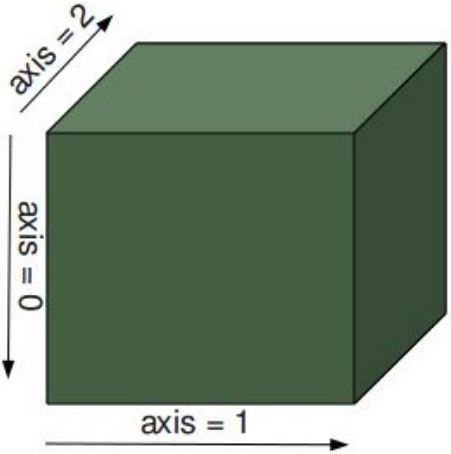
\includegraphics[scale=0.22]{pics/array}
            {\tiny\url{https://www.python-kurs.eu/numpy_arrays_erzeugen.php}}
        \end{figure}
    \end{block}
    
    \pagebreak
    
    \begin{block}{Indizierung und Slicing}
        \begin{itemize}
            \item Für jede Dimension: "[start:stop:step]"
        \end{itemize}
        \begin{minipage}{0.45\linewidth}
            \begin{lstlisting}
        print(x[0])  # 1
        print(x[2:-1])  # [3 4 5 6 7]
            \end{lstlisting}
        \end{minipage}
        \begin{minipage}{0.4\linewidth}
            \begin{lstlisting}
    print(x[:4])  # [1 2 3 4]
    print(x[::2])  # [1 3 5 7]
            \end{lstlisting}
        \end{minipage}
        \\Siehe {\footnotesize\url{https://numpy.org/doc/stable/user/basics.indexing.html}}
    \end{block}
    \vspace*{-3mm}
    \begin{block}{2D Beispiel}
        \begin{minipage}{0.4\linewidth}
        \begin{lstlisting}
    z = np.array([
        [11, 12, 13, 14, 15],
        [21, 22, 23, 24, 25],
        [31, 32, 33, 34, 35],
        [41, 42, 43, 44, 45],
        [51, 52, 53, 54, 55]])
        \end{lstlisting}
        \end{minipage}
        \begin{minipage}{0.5\linewidth}
        \begin{lstlisting}
    print(z[2, 2])  # 33
    print(z[3:, :-1])  # [[41 42 43 44]
                 # [51 52 53 54]]
    print(z[:, 3])  # [14 24 34 44 54]
    print(z[::3, ::-1])  # [[15 14 13 12 11]
                  # [45 44 43 42 41]]
        \end{lstlisting}
        \end{minipage}
    \end{block}
    
    \pagebreak
    
    \begin{block}{Array Initialisierungen}
    \begin{lstlisting}
    np.array() # direkt
    np.ones(shape) # Einsen
    np.zeros(shape) # Nullen
    np.full(shape, value) # Array voll mit 'value'
    # gleichverteilte Werte aus [start, stop), analog zu range()
    np.arange([start,] stop[, step])
    # 'num' viele gleichverteilte Werte aus [start, stop] bzw. [start, stop)
    np.linspace(start, stop[, num=50][, endpoint=True]) 
    np.random.rand(*shape) # Zufaellige floats aus [0,1]
    np.random.randint([start,] stop, shape) # Zufaellige integer aus [start, stop)
    \end{lstlisting}
    $\dots$ und viele weitere (siehe auch  {\footnotesize\url{https://numpy.org/doc/stable/reference/routines.array-creation.html}})    
    \end{block}
    
    \pagebreak
    
    \begin{block}{Array Operationen}
        \begin{itemize}
            \item Generell \textbf{elementweise}
        \end{itemize}
        \begin{minipage}{0.45\linewidth}
        \begin{lstlisting}
        a = np.array([[1, 2, 3], [4, 5, 6]])
        print(a + 10)  # [[11 12 13]
                   # [14 15 16]]
        print(a ** 2)  # [[ 1  4  9]
                  # [16 25 36]]
        \end{lstlisting}
        \end{minipage}
        \begin{minipage}{0.45\linewidth}
        \begin{lstlisting}
        b = np.full((2, 3), 3)
        print(a - b)  # [[-2 -1  0]
                  # [ 1  2  3]]
        print(a * b)  # [[ 3  6  9]
                  # [12 15 18]]
        \end{lstlisting}
        \end{minipage}
        \begin{itemize}
            \item Oder spezielle algebraische Methoden\\(z.B. Matrixmultiplikation)
        \end{itemize}
        \begin{lstlisting}
        c = np.transpose(a)  # Transponierte Matrix
        print(np.matmul(a, c))  # [[14 32]
                           # [32 77]]
        \end{lstlisting}
    \end{block}
    
    \pagebreak
    
    \vspace*{3mm}
    \begin{itemize}
        \item Lassen sich Arrays unterschiedlicher shape miteinander kombinieren?
    \end{itemize}
	\begin{block}{Broadcasting - Idee}
		\begin{itemize}
			\item Beschreibt wie Arrays unterschiedlicher Form während arithmetischen Operationen behandelt werden.
			\item Unter bestimmten Einschränkungen wird das kleinere Array auf das größere Array "übertragen" (broadcast), sodass ihre Formen kompatibel sind.
			\item Skalare werden immer auf das gesamte Array übertragen
		\end{itemize}
	\end{block}

	\pagebreak

	\begin{block}{Broadcasting - Regeln}
		\begin{itemize}
			\item Beim Operieren auf zwei Arrays werden ihre shapes elementweise von hinten nach vorne verglichen.
			\item Zwei Dimensionen sind kompatibel, wenn
			\begin{itemize}
				\item[$1)$] sie gleich sind.
				\item[$2)$] eine von ihr $1$ ist.
			\end{itemize}
			\item Die Größe des resultierenden Arrays ist die maximale Größe entlang jeder Dimension der Eingabearrays.
			\item Arrays müssen nicht den gleichen Rang haben um broadcast-kompatibel zu sein, es müssen nur alle elementweisen Vergleiche der Dimensionen kompatibel sein.
		\end{itemize}
	\end{block}
	
	\pagebreak
	
	\begin{block}{Broadcasting - Beispiele}
		\hspace{5mm}
		\begin{minipage}{0.4\textwidth}
			\begin{tabular}{|rr|} \hline
			$A$ (3d): & $2\times 3\times 5$ \\
			$B$ (1d): & $1$ \\
			$A\bullet B$ (3d): & $2\times 3\times 5$ \\ \hline
			%
			$A$ (2d): & $5\times 4$ \\
			$B$ (1d): & $4$ \\
			$A\bullet B$ (2d): & $5\times 4$ \\ \hline
			%
			$A$ (3d): & $15\times 3\times 5$ \\
			$B$ (3d): & $15\times 1\times 5$ \\
			$A\bullet B$ (3d): & $15\times 3\times 5$ \\ \hline
			%
			$A$ (3d): & $15\times 3\times 5$ \\
			$B$ (2d): & $3\times 5$ \\
			$A\bullet B$ (3d): & $15\times 3\times 5$ \\ \hline
			\end{tabular}
		\end{minipage}
		\hspace{5mm}
		\begin{minipage}{0.4\textwidth}
			\begin{tabular}{|rr|} \hline
			$A$ (2d): & $2\times 1$ \\
			$B$ (2d): & $2\times 3$ \\
			$A\bullet B$ (2d): & $2\times 3$ \\ \hline
			%
			$A$ (2d): & $6\times 1$ \\
			$B$ (3d): & $7\times 1\times 5$ \\
			$A\bullet B$ (3d): & $7\times 6\times 5$ \\ \hline
			%
			$A$ (1d): & $3$ \\
			$B$ (1d): & $5$ \\
			$A\bullet B$ (---): & \textit{error} \\ \hline
			%
			$A$ (2d): & $2\times 1$ \\
			$B$ (3d): & $8\times 4\times 3$ \\
			$A\bullet B$ (---): & \textit{error} \\ \hline
			\end{tabular}
		\end{minipage}
	\end{block}
\end{frame}

%%%%%%%%%%%%%%%%%%%%%%%%%%%%%%%%%%%%%%%%%%%%%%%%%%%%%%%%%%%%%%%%%%%%%%%%%%%%%%%%%%%%%%%%%
%%%%%%%%%%%%%%%%%%%%%%%%%%%%%%%%%%%%%%%%%%%%%%%%%%%%%%%%%%%%%%%%%%%%%%%%%%%%%%%%%%%%%%%%%
%%%%%%%%%%%%%%%%%%%%%%%%%%%%%%%%%%%%%%%%%%%%%%%%%%%%%%%%%%%%%%%%%%%%%%%%%%%%%%%%%%%%%%%%%
\section{Graphiken mit Matplotlib}
\begin{frame}[fragile]{Graphiken mit \tt{Matplotlib}}
	\begin{itemize}
		\item Python-Bibliothek zum Plotten (Daten, Graphen, Bilder etc.)
		\item Untermodel \tt{pyplot} als Schnittstelle zur Plot-Bibliothek von Matplotlib
	\end{itemize}	
	\begin{lstlisting}
		import matplotlib.pyplot as plt
	\end{lstlisting}
	\begin{itemize}
		\item Alle \tt{pyplot}-Funktionen beziehen sich auf eine Abbildung (figure) und Plot-Bereich (axes)
		\item \tt{pyplot} legt automatisch \textit{eine} figure im Hintergrund an, sodass man sich bei einfachen Plots darum nicht kümmern muss
		\item Abbildungen werden angezeigt sobald \tt{plt.show()} aufgerufen wird
	\end{itemize}
\end{frame}

\begin{frame}[fragile]{Plotten mit \tt{pyplot}}
	\begin{block}{\tt{plt.plot}}
	\begin{itemize}
		\item Zum plotten von $(x,y)$-Datenpunkten
		\item Arbeitet auf Listen
		\begin{itemize}
			\item Eine einzelne Liste wird als $y$-Werte interpretiert, mit ihren Indizes als $x$-Werte
			\item Zwei Listen werden als $y$- und $x$-Werte interpretiert
		\end{itemize}
		\item Unterstützt Format-Parameter zum Anpassen der Darstellung
		\begin{itemize}
			\item Linienstil
			\item Darstellung der diskreten Werte
			\item Farbe
		\end{itemize}
	\end{itemize}
	\end{block}
\end{frame}

\begin{frame}[fragile]{\tt{plt.plot} -- Beispiele}
	\begin{minipage}[t]{0.45\textwidth}
		\begin{itemize}
			\item Einzelne Liste als $y$-Werte (implizite $x$-Werte)
		\end{itemize}
		\begin{lstlisting}
	import matplotlib.pyplot as plt
	
	plt.plot([-1, -4.5, 16, 23, 15, 59])
	plt.show()
		\end{lstlisting}
		\begin{figure}
			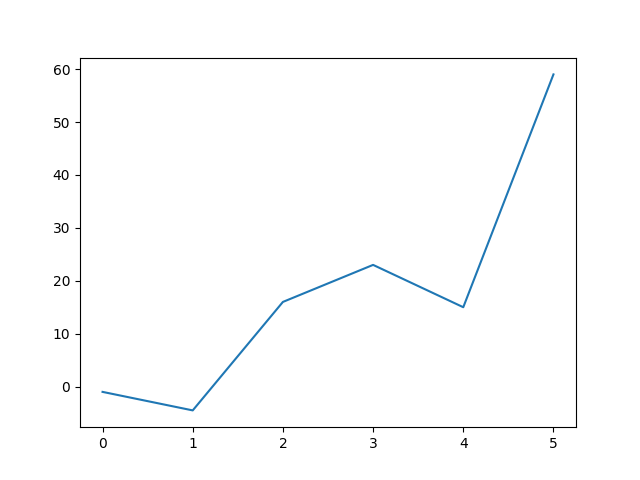
\includegraphics[width=0.9\textwidth]{pics/plot1}
		\end{figure}
	\end{minipage}
	\begin{minipage}[t]{0.45\textwidth}
		\begin{itemize}
			\item Zwei Listen als explizite $x$- und $y$-Werte
		\end{itemize}
		\begin{lstlisting}
	xs = [0, 2, 4, 6, 8]
	ys = [-2, -1, 0, -1, -2]
	plt.plot(xs, ys)
	plt.show()
		\end{lstlisting}
		\begin{figure}
			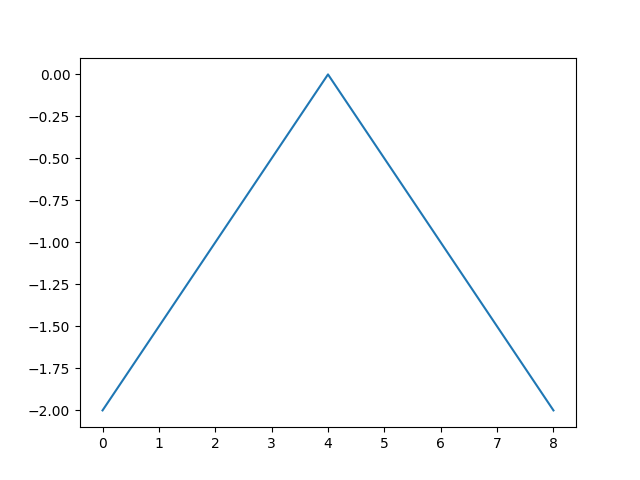
\includegraphics[width=0.9\textwidth]{pics/plot2}
		\end{figure}
	\end{minipage}
\end{frame}

\begin{frame}[fragile, allowframebreaks]{\tt{plt.plot} -- Formatierung}	
	\begin{itemize}
		\item Format-Parameter enthält \tt{[marker][line][color]}
	\end{itemize}
	\begin{minipage}[t]{0.45\textwidth}
		\begin{itemize}
			\item \verb|'^r'| $\rightarrow$ rote Dreiecke ohne Linie
		\end{itemize}
		\begin{lstlisting}
	plt.plot([-1, -4.5, 16, 23, 15, 59], '^r')
	plt.show()
		\end{lstlisting}
		\begin{figure}
			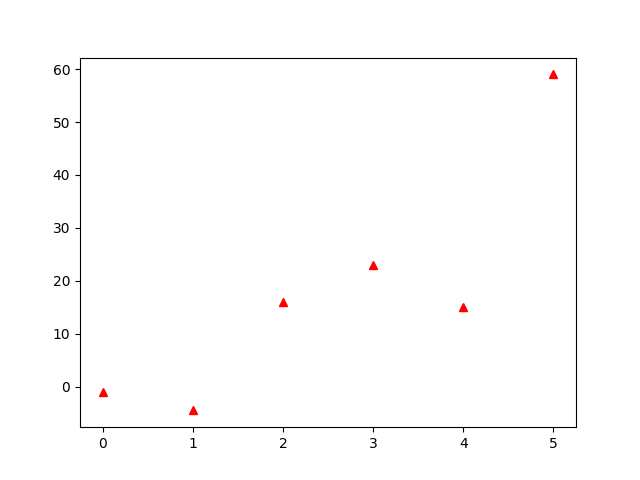
\includegraphics[width=0.9\textwidth]{pics/plot3}
		\end{figure}
	\end{minipage}
	\begin{minipage}[t]{0.45\textwidth}
		\begin{itemize}
			\item \verb|'x:k'| $\rightarrow$ schwarze Kreuze mit gepunkteter Linie
		\end{itemize}
		\begin{lstlisting}
	plt.plot([-1, -4.5, 16, 23, 15, 59], 'x:k')
	plt.show()
		\end{lstlisting}
		\begin{figure}
			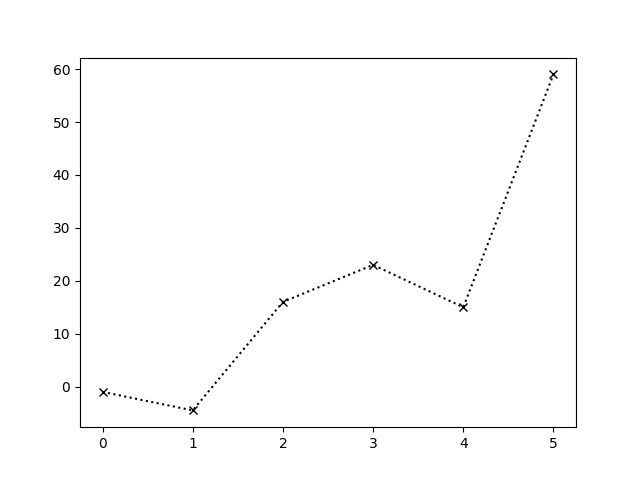
\includegraphics[width=0.9\textwidth]{pics/plot4}
		\end{figure}
	\end{minipage}
	
	\pagebreak
	
	\vspace*{-2mm}
	\begin{minipage}[t]{0.45\textwidth}
		\begin{tabular}{|l|l|} \hline
		\textbf{character} & \textbf{marker} \\ \hline
		\verb|.| & point \\ \hline
		\verb|,| & pixel \\ \hline
		\verb|o| & circle \\ \hline
		\verb|v| & triangle down \\ \hline
		\verb|^| & triangle up \\ \hline
		\verb|<| & triangle left \\ \hline
		\verb|>| & triangle right \\ \hline
		\verb|1| & tri down \\ \hline
		\verb|2| & tri up \\ \hline
		\verb|3| & tri left \\ \hline
		\verb|4| & tri right \\ \hline
		\end{tabular}
	\end{minipage}
	\begin{minipage}[t]{0.45\textwidth}
		\begin{tabular}{|l|l|} \hline
		\textbf{character} & \textbf{marker} \\ \hline
		\verb+s+ & square \\ \hline
		\verb+p+ & pentagon \\ \hline
		\verb+*+ & star \\ \hline
		\verb+h+ & hexagon1 \\ \hline
		\verb+H+ & hexagon2 \\ \hline
		\verb|+| & plus \\ \hline
		\verb+x+ & cross \\ \hline
		\verb+D+ & diamond \\ \hline
		\verb+d+ & thin diamond \\ \hline
		\verb+|+ & vertical line \\ \hline
		\verb+_+ & horizontal line \\ \hline
		\end{tabular}
	\end{minipage}
	
	\pagebreak
	
	\vspace*{-2mm}
	\begin{minipage}{0.45\textwidth}
		\begin{tabular}{|l|l|} \hline
		\textbf{character} & \textbf{line style} \\ \hline
		\verb|-| & solid \\ \hline
		\verb|--| & dashed \\ \hline
		\verb|-.| & dash-dot \\ \hline
		\verb|:| & dotted \\ \hline
		\end{tabular}
	\end{minipage}
	\begin{minipage}{0.45\textwidth}
		\begin{tabular}{|l|l|} \hline
		\textbf{character} & \textbf{color} \\ \hline
		\verb|b| & blue \\ \hline
		\verb|g| & green \\ \hline
		\verb|r| & red \\ \hline
		\verb|c| & cyan \\ \hline
		\verb|m| & magenta \\ \hline
		\verb|y| & yellow \\ \hline
		\verb|k| & black \\ \hline
		\verb|w| & white \\ \hline
		\end{tabular}
	\end{minipage}
	
	\pagebreak
	
	\vspace*{-2mm}
	\begin{itemize}
		\item (Weitere) Argumente zur Formatierung können auch direkt an die \tt{plot}-Funktion übergeben werden:
	\end{itemize}
	
	\vspace{-2mm}
	\begin{minipage}{0.4\textwidth}
		\begin{lstlisting}
	plt.plot(xs, ys,
	      color='green',
	      marker='o',
	      linestyle='dashed',
	      linewidth=2.5,
          markersize=12,
	      label='line xy', ...)
	plt.legend()  # for the label
	plt.show()
		\end{lstlisting}
	\end{minipage}
	\begin{minipage}{0.5\textwidth}
		\begin{figure}
			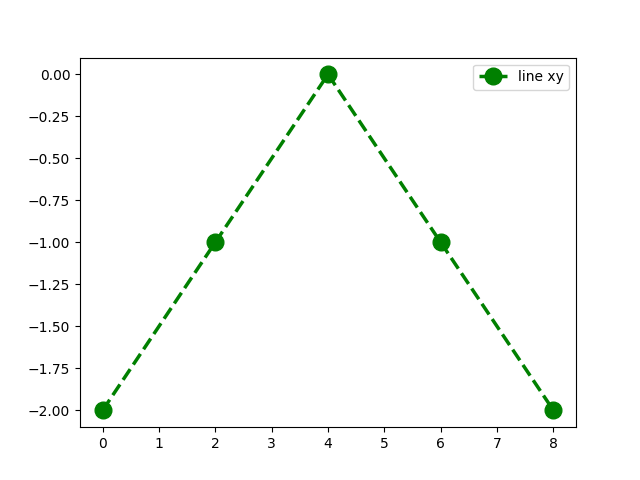
\includegraphics[width=0.9\textwidth]{pics/plot5}
		\end{figure}
	\end{minipage}
\end{frame}

\begin{frame}[fragile]{Streudiagramme (Punkt-Plots)}
	\begin{itemize}
		\item Mittels \tt{plt.plot}, indem die Verbindungslinien ausgeblendet werden
		\item Flexibler: \tt{plt.scatter}\\ $\rightarrow$ Farbe und Größe der Markierungen (und weiteres) können \textit{individuell} gesetzt werden
	\end{itemize}
	\vspace{-2mm}
	\begin{minipage}{0.45\textwidth}
		\begin{lstlisting}
	plt.scatter(points_x, points_y, s=25
	         c=points_color, alpha=0.5)
	plt.plot(centroids_x, centroids_y,
	      marker='x', markersize=15,
	      markeredgecolor="black",
	      linestyle="None")
	plt.show()
		\end{lstlisting}
	\end{minipage}
	\begin{minipage}{0.5\textwidth}
		\begin{figure}
			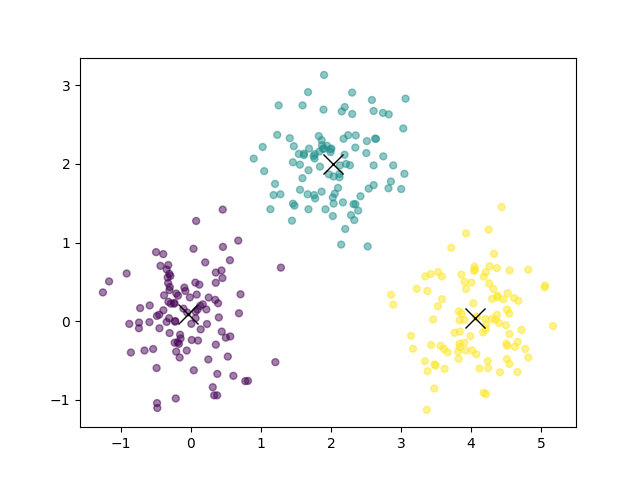
\includegraphics[width=0.95\textwidth]{pics/scatter}
		\end{figure}
	\end{minipage}
\end{frame}

\begin{frame}[fragile, allowframebreaks]{\tt{figure} -- Formatierung}
	\begin{itemize}
		\item Achsenbeschriftungen mittels\\ \tt{plt.xlabel('x-Achse')} und \tt{plt.ylabel('y-Achse')}
		\item Wertebereich der Achsen anpassen mittels\\ \tt{plt.axis([xmin, xmax, ymin, ymax])} \\ oder Achsen ausblenden mittels \\ \tt{plt.axis("off")}
		\item Titel der Abbildung mittels \tt{plt.title('Titel')}
	\end{itemize}
	
	\framebreak
	
	\vspace*{1mm}
	\begin{block}{\tt{plt.subplot}}
		\begin{itemize}
			\item Mehrere Abbildungen in einer \tt{figure}
			\item Argumente: \tt{plt.subplot(rows, cols, pos)} \\ $\rightarrow$ Aufteilung in \textit{rows} Zeilen und \textit{cols} Spalten\\ $\rightarrow$ Untergraph an der Position \textit{pos} (Index von 1 bis \textit{rows}$*$\textit{cols})
% 			\item Abstände und Ausrichtung mittels \tt{plt.subplots\textunderscore adjust()}
		\end{itemize}
	\end{block}
	\vspace*{-2mm}
	\begin{minipage}{0.48\textwidth}
		\begin{lstlisting}
	colors = ['green', 'red', 'yellow', 'blue']
	plt.suptitle("Multiple subfigures")
	for i, c in enumerate(colors):
    	plt.subplot(2, 2, i+1)
    	plt.plot(xs, ys, color=c)
    	plt.title("Subplot {}/4".format(i+1))
	plt.subplots_adjust(hspace=0.4)
	plt.show()
		\end{lstlisting}
	\end{minipage}
	\begin{minipage}{0.51\textwidth}
		\begin{figure}
			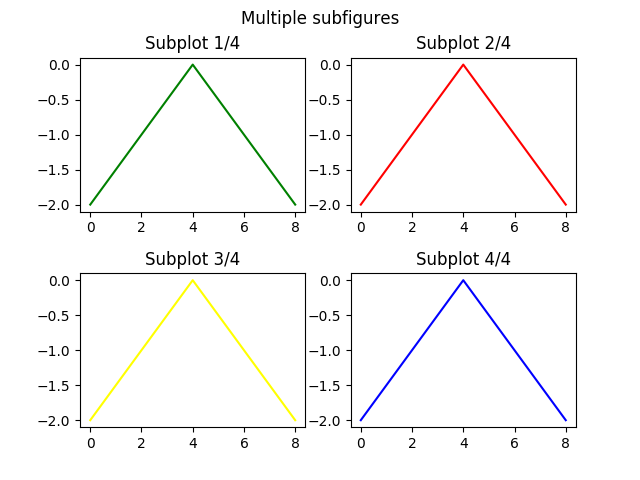
\includegraphics[width=0.95\textwidth]{pics/subplots}
		\end{figure}
	\end{minipage}
\end{frame}

\begin{frame}[fragile]{Bilder}
    \vspace*{1mm}
	\begin{block}{\tt{plt.imshow}}
		\begin{itemize}
			\item Darstellen von Bildern auf einem 2D-Raster
			\item Input Daten 2D $\rightarrow$ Zeilen und Spalten des Bildes
			\item Optionale dritte Dimension für RGB(A) Werte
		\end{itemize}
	\end{block}
	\vspace{-2mm}
	\begin{minipage}{0.48\textwidth}
		\begin{lstlisting}
	# 'imgs' enthaelt sechs 28x28 Bilder
	for i in range(6):
    	plt.subplot(2, 3, i+1)
    	# mit grauer colormap
    	plt.imshow(imgs[i], cmap="gray")
    	# ohne Achsen
    	plt.axis("off")
	plt.show()
		\end{lstlisting}
	\end{minipage}
	\begin{minipage}{0.51\textwidth}
		\begin{figure}
			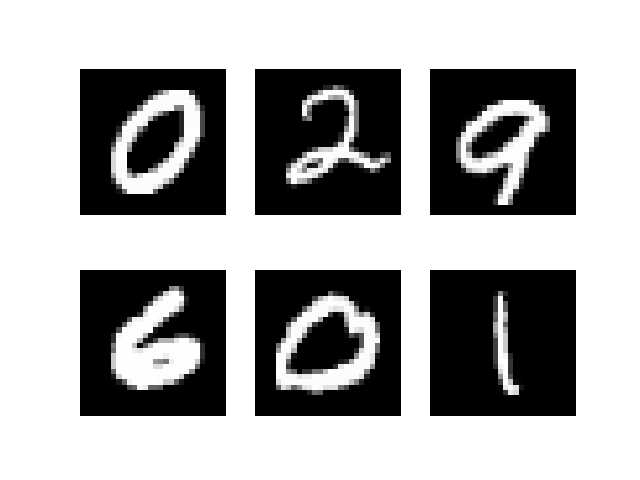
\includegraphics[width=\textwidth]{pics/imshow}
		\end{figure}
	\end{minipage}	
\end{frame}

\end{document}